\documentclass[a4paper,oneside,12pt,openany]{memoir}
\usepackage{fullpage}
\usepackage{graphics}
\usepackage[compact]{titlesec}
\usepackage[left=35mm, right=24mm, top=24mm, bottom=24mm]{geometry}
\setlength{\parindent}{0cm}
\setlength{\parskip}{0.4cm}
\setcounter{tocdepth}{3}
\maxsecnumdepth{subsection}
\chapterstyle{section}
\tightlists
\begin{document}
\frontmatter
\thispagestyle{empty}
\vspace*{\fill}
\begin{center}

{\Large \textsc{Electronics and Computer Science}} \\[0.3cm]
{\Large Faculty of Physical and Applied Sciences} \\[0.3cm]
{\Large University of Southampton} \\[2cm]

{\Large Thomas A. E. Smith} \\[0.2cm]
taes1g09@ecs.soton.ac.uk\\[0.3cm]
{\large \today} \\[1.5cm]

\textbf{\LARGE Intelligent Procedural Content Generation\\[0.2cm] for Computer Games} \\ [5cm]

{\Large Project supervisor: E. Gerding - eg@ecs.soton.ac.uk} \\[0.3cm]
{\Large Second examiner: C. Cirstea - cc2@ecs.soton.ac.uk} \\[1.5cm]

{\large A project progress report submitted for the award of} \\[0.3cm]
{\large MEng Computer Science with Artificial Intelligence}

\end{center}
\vspace*{\fill}

\pagebreak
\vspace*{\fill}
\begin{abstract}
Increasingly, as the demand for ever larger and more varied computer game environments grows, procedural content generation (PCG) is used to ensure that content remains `fresh'. However, many of the opportunities to use these systems to generated truly personalised content have so far been largely overlooked. When content is generated manually or algorithmically during the design phase of a game, it can only be created according to the designer�s expectations of the players� needs. By instead generating content during the execution of the game, and using information about the player(s) as one of the system�s inputs, PCG systems should be able to produce more dynamic experiences that can be far more tailored to enhance individual players' experiences than anything manually created. Much has been written about the generation of player models for the purposes of adaptivity or dynamic difficulty adjustment (DDA), and literature exists examining the problem of generating satisfying game environments via challenge adjustment. This project looks at combining these two fields to create an intelligent PCG system (IPCG) that is capable of monitoring players' progress and dynamically generating upcoming challenges to best suit their abilities. 




\end{abstract}
\vspace*{\fill}
\pagebreak

\tableofcontents*
% \pagebreak
\mainmatter
\chapter{Project Description}
The aim of this project is to investigate the use of IPGC in computer games, by looking at existing products, research in related areas and constructing a minimal prototype. Due to the increasing demand for both detail and variety within computer game environments, various aspects of in-game content are now often generated procedurally (that is, algorithmically rather than manually), using techniques that are frequently just refinements of algorithms used in the early days of computing, for games such as Elite (Acornsoft 1984).
However, one of the strengths of PCG is that (within reasonable limits) it may be performed at runtime, allowing it to also use information about the player in order to dynamically generate content on-the-fly in response to the player's actions. In general, this will involve making use of algorithms from the field of artificial intelligence in order to evaluate the information available and condense it to a form suitable for input to a PCG system; hence such systems might reasonably be termed `intelligent' procedural content generators (IPCG).
As shown later in the Literature Review and Background Research sections, IPCG techniques can be applied to many different scenarios. For the purposes of this project, the problem will be restricted to using IPCG for DDA in basic 2D platformer levels. 




\section{Requirements}
The main aim of the project requirements will be to constrain the problem to an achievable scale, and inform future evaluation of the final solution. In this instance, the functional requirements are generic to any IPCG system (with refinements specific to this problem in brackets, like so), while the non-functional requirements are constraints that should serve to encourage feasibility and quality.



\subsection{Functional}
In order to properly implement IPCG, the system should:
\begin{itemize}[-]
\item present the user with an interactive game environment (basic 2D platformer)
\item record data on the player's behaviour (in this case, performance)
\item evaluate this data according to specific criteria (a trained classifier)
\item form a model of some aspect of the player (skill relative to current difficulty)
\item use this model to inform further PCG activities (level chunk generation)
\end{itemize}
\subsection{Non-Functional}
In order to remain at a manageable scale, the system should:
\begin{itemize}[-]
\item be written in Java
\item be confined to 2D
\item be presented as a basic platformer
\item limit the user to move and jump actions
\end{itemize}
but also:
\begin{itemize}[-]
  \item remain responsive
  \item properly maintain the challenge of generated content
\end{itemize}
\chapter{Project Background}
	procedural content for many purposes (music strucure enemies textures)
	DDA resident evil
	use in existing games (valve, infintie mario)
	IPCG for difficulty, preference(fun), exploration


Procedural Content Generators have been used since the early days of gaming. Elite <one of the first great Y> had <stats>, all procedurally generated. These technique were required, as it was not possible to store the full data about that many unique planets on the distribution media that was availabe at the time. As technologies improved; focus shifted more towards hand-crafted environments as it was easier to ensure that these provided value and did not feel sparse \cite{elements game}. However, with the further progress of technology attention has returned to procedural generation. Modern game worlds contain vast amounts of detail, and procedural content generation algorithms are ideally suited to producing large numbers of variations on a theme \cite{speedtree}, <expand> clouds textures sounds. Producing each of these items individually by hand would take many hours of labour and much disk space, but by defining specific sub elements and assmbly rules, variation can be almost endlessly reused. Not only used for cosmetics now either. Minecraft, infinite Mario?

Another facet of game design that has benefited <introduction to DDA>. Previously, games had been limited to specific discrete difficulties as defined at production time. However, these (can have been) considered to be overly restrictive - typically, if a games is begun with a certain difficulty it is difficult to later change; and this also alienates players that are unfamiliar with the standards or uncertain how to classify themselves. Furthermore, since game difficulty is typically a continuous function of multiple parameters <stuff>. Typically, DDA is achieved by altering values that are hidden from the player, such as enemy health, accuracy, or the amount of ammo and healthkits available in the world \cite{hamlet}. Often, the intention is to do this invisibly, and merely ensure that the player remains optimally challenged. By manipulating values behind the scenes, it is possible to ensure that the player is neither overchallenged (leading to frustration), or underchallenged, leading to boredom \cite{flow}. As DDA systems are given more control over additional aspects of the game environment, they can begin to enter the realm of PCG, fundamentally(?) altering the stucture and pacing of the player's experience. In the game Left 4 Dead, there is an 'AI Director' that is capable of estimating the <intensity> of each player's situation, and dynamically altering the generation of enemies of various types in order to ensure that the general flow of the game is kept exciting, <following build up, panic and calm phases> \cite{valve}. In Left 4 Dead 2, the director has additional control, and is able to vary the stucture of the level (something about the placement of ammo)(possible additional cite).

Typically, PCG is used in an offline manner, taking input only from a random seed. DDA, in contrast, uses information about the players' actions as an input,

IPCG can be (and has been) used for a wide range of purposes, almost as varied as PCG itself. As one of the key challenges in game design is maintaining players' engagement with the game via enhancing immersion and controlling flow\cite{flow}, it is unsurprising that many of the existing applications of IPCG are used for these reasons.<<send to front> One of the most well-known such applications is used in Valve's games Left 4 Dead and Left 4 Dead 2. Known as the `AI Director', the system monitors the ``emotional intensity'' of each players' gameplay experience, and manipulates the game environment in order to control pacing and maintain flow\cite{valve}. 

\chapter{Literature Review}
\section{}
\chapter{Proposed System}
\section{Overview}
Following the separation of concerns (SoC) design practice, the project may easily be modularised into three principle components: a `host' or base module, an adaptive PCG system, and a means of taking data about the player and converting it into a model usable by the PCG. The proposed flow of information is shown in \fref{Figure:dataflow}.

\begin{figure}[htbp]
  \centering
%   \scalebox{0.6}{\input{toyplot}}
  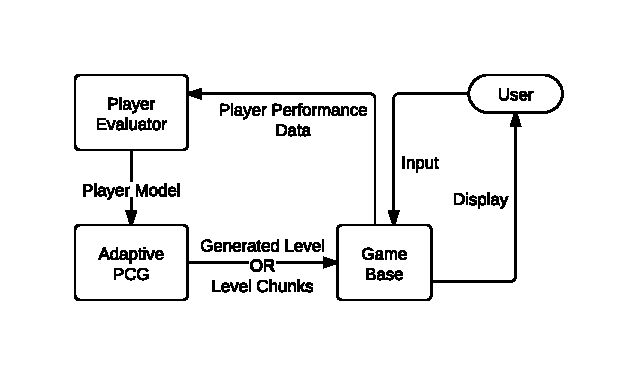
\includegraphics{system}
  \caption{Data flow in proposed system.}
  \label{Figure:dataflow}
\end{figure}
\subsection{Game Base}
A simple 2D platformer engine. This module should handle all input and rendering activity, and ought to be created following the MVC architecture. In addition to presenting the user with the output of the IPCG system, the Base module should provide the basic input handling, physics and game functionality necessary to play the platformer, while also harvesting multiple types of information about the players performance for the Evaluator module. 
\subsection{Adaptive PCG}
An adaptable 2D platforming level generator. Building on the work of <nop>, this module should maintain a context-free grammar (CFG) of obstacles available, along with weights representing the estimated challenge of each element (terminal obstacle or combination). By taking these weights into account when deriving a string of obstacles from the CFG, sequences of a desired difficulty can be produced - or alternatively, the estimated challenge of existing sequences may be evaluated. A PCG system designed in this way should be able to generate entire levels `offline', by maintaining pre-determined maxima and local variations in difficulty, but should also be capable of generating levels on-the-fly, by ensuring that short-term future difficulty levels match those requested by the Evaluator.
\subsection{Player Evaluator}
A <nop> classifier. Given the varied inputs from the Base module, the Evaluator should form a belief about the player's skill relative to the current challenge of the level. By running the player's data through a previously-trained classifier, this module should obtain a model that can be passed to the PCG module and acted upon.
 
% evaluator
%  custom data
%  list of possible data
%  expect to initially be able to use k-means to disretise
%  PCA for visualisation?
%  One-vs-All SVM
%  current belief fed back into pcg
 \section{Approach}
The modules above are presented in logical order of development: none of the IPCG system will be testable without the Base program (which can be tested standalone if given a hand-crafted level), but the PCG may be run and tested using specimen models, and finally the Evaluator can be tested once the other systems are in place.
\subsection{Classifier Training}
 The development of the classifier will involve initially collecting data on as many potentially relevant features of the player's performance as possible, and then performing principle component analysis (PCA) upon the data-set in order to identify the maximally variant features. These can then be retained and used as the input to a K-means discretisation algorithm, which can be used to train a One-vs-All SVM classifier. 
 \section{Justification}
 %Goals: As specified above, an intelligent PCG should consist of two sub- systems: an evaluator and its companion generator. The aim of the project will be to create a simple game-like application that uses an IPCG system to produce dynamically variable content based on the player�s behaviour. I will begin by creating a variable PCG that is able to produce content based on specimen player models, and then use environments created in this way to create and tune a player evaluator for further generation.
%Scope: In order to attempt to ensure that the project goals remain achiev- able, the scope should be restricted to the simplest possible system. Based on inital inspection of the problem space and existing literature, it appears that this would be adjustment due to player skill in a 2D platforming envi- ronment. The project will be coded in Java, as that comprises the majority of my recent coding experience, and it has a wealth of 2D graphics drawing support which will simplify the less-relevant areas of coding. Similarly, many of the peripheral components traditionally included in computer games are irrelevant to the project and will not be needed.
 
 \section{Possible Extensions}
\cite{Hunicke:2005:CDD:1178477.1178573}
\cite{Nitsche:1428967}
\chapter{Plan of remaining work}

\section{Gantt Chart}
\bibliography{IPCG}{}
\bibliographystyle{plain}
% And if you need to split it up use %\section{section name}

% \appendix
% \chapter{Appendix}

\end{document}


The body of the progress report must not exceed 3,000 words. This is about 10 A4 pages of standard-spaced text.

The progress report should provide:

An enhanced project description (development of the brief above)
A report on the background research and literature search
The proposed final design of the system or experiment
A justification for the approach
An account of the work to date
A plan of the remaining work
An estimate of any support required to complete the project
A Gantt chart showing the schedule of both completed and remaining work
The presentation of the progress report must conform with the Project Report Standards shown below.

For electronic submission it is necessary to submit 2 PDF files via the ECS Handin System.

the progress report in PDF format for the Archive.
shorter version of the progress report in PDF format for Plagiarism Checking.
Following this, one paper copy of the report and a copy of the electronic submission acknowledgement sheet are submitted to Zepler reception.

Note that early submission of the progress report may be appropriate if a case for significant facilities or financial support needs to be made.

The progress report contributes about 10% of the final assessment.

Failure to submit a progress report in the approved format by the deadline will result in its part of the project mark being subject to a 10% penalty per working day late. A progress report submitted more than 5 days late will result in the relevant part of the project mark being set to zero.



\end{document}
